\documentclass[spanish,12pt,letterpaper]{article}
\usepackage[spanish, es-tabla]{babel}%paquete para idiomas
\usepackage[utf8]{inputenc}%paquete para la codificacion
\usepackage{color}
\usepackage[usenames,dvipsnames]{xcolor}
\usepackage{graphicx}
\usepackage{minted}
\usepackage{float}

\title{\textcolor{blue}{Editor de textos LaTex}}
\date{\today}

\thispagestyle{empty}

\begin{center}


\includegraphics[width=0.5\textwidth]{logoTECdeMtyColor.jpg}\\
\vspace{2cm}
\Large \sc  Tecnológico de Monterrey\\
	            Campus Guadalajara


\vspace{2cm}
\huge \bf
\emph{Análisis exploratorio de datos: \textit{Driving Behavior Challenge}}
\end{center}

\vspace{2cm}

\rightline{\Large Edgar Daniel Acosta Rosales | A01276214}
\rightline{\Large Diana Guadalupe García Aguirre | A01276380}
\rightline{\Large José Herón Samperio León | A01276217}
\rightline{\Large David Alejandro Velázquez Valdéz | A01632648}

\vspace{1.5cm}
\rightline{\textbf{Inteligencia artificial avanzada para la ciencia de datos I}}
\rightline{Dr. Gildardo Sánchez Ante}
\rightline{Dra. Brenda Ivette García Maya}
\rightline{Dr. Javier Mauricio Antelis}
\rightline{Dr. Alberto De Obeso Orendáin}
\vspace{1cm}

\begin{center}
	\large \bf  29 de agosto del 2022
\end{center}

\vspace{3cm}
\begin{document}



\tableofcontents
\listoffigures
\listoftables

\newpage

\section{Resumen}

\textsc Uno de los principales factores que influyen en la ocurrencia de accidentes de tráfico es un comportamiento de conducción agresivo. Según lo informado por la \textit{AAA Foundation for Traffic Safety}, en el 55.7 por ciento de los accidentes de tráfico que fueron registrados a lo largo de cuatro años |es decir, 106727 accidentes fatales|, los conductores involucrados presentaron una o más conductas de conducción agresivas. Con base en esto, se realizará un modelo de \textbf{clasificación supervisada} que, además de describir las métricas de los tipos de comportamiento que se reflejan en los datos recopilados de tres pruebas de manejo, ayudará a predecir el momento en el que los automovilistas, debido a sus técnicas de manejo, se encuentren en riesgo de sufrir un accidente de tráfico fatal. \\

\section{Antecedentes e introducción}

\textsc Ion Cojocaru, Stefan Popescu y Cristian Mihaescu, estudiantes de la Universidad de Craiova, en Rumania, llevaron a cabo un experimento de conducción, en el que dos personas: un conductor y su copiloto, se subieron a un automóvil y, a lo largo de tres periodos de, aproximadamente, diez minutos, trabajaron de manera conjunta: mientras uno conducía el vehículo en un estilo determinado, el otro medía con una aplicación de Android, dos veces por segundo, los valores registrados por el giroscopio y el acelerómetro del dispositivo en tres dimensiones del plano, para asociar dichos registros al estilo de manejo correspondiente. La labor de este último se concentraba en mantener el teléfono quieto y estable durante la toma de valores.\\

\textsc Los datos recopilados se centran en registrar conductas tales como excesos de velocidad, frenados y giros bruscos. Los autores del experimento aseguran que el origen de la idea de crear una aplicación que realice tales registros, es el hecho de que la gran mayoría de las personas en la actualidad posee un teléfono inteligente y, de establecerse modelos de predicción adecuados, podría desarrollarse una aplicación que ayude a reducir la cantidad de accidentes fatales. \\

\textsc En la actualidad, la problemática antes descrita se encuentra cargada en la plataforma más grande de científicos de datos: Kaggle, una subsidiaria de Alphabet Inc., la compañía dueña de Google, el buscador más popular del mundo. En dicha plataforma se encuentran cargados los datos antes mencionados y el reto asociado se halla abierto y en espera de propuestas de modelos, de cualquier usuario del mundo, que ayuden a predecir con la mayor precisión posible las conductas de conducción agresivas con datos nuevos. \\

\section{Análisis exploratorio de los datos}

\textsc Para efectos de la obtención, entrenamiento y prueba de cualquier modelo de aprendizaje automático, es necesario contar con datos. En el caso que analizaremos, se cuenta con dos conjuntos de datos, uno de entrenamiento llamado \verb|train_motion_data.csv| con 3644 observaciones y uno de prueba llamado \verb|test_motion_data.csv| con 3084 observaciones, ambos documentando ocho variables, siendo siete de ellas variables independientes y una de ellas dependiente, llamada \verb|Class|, que define cuál es el tipo de comportamiento descrito por cada evento registrado. La llamamos dependiente porque asumiremos que las demás variables influyen en ella. \textit{A posteriori}, usaremos el conjunto de prueba para verificar que nuestro modelo sea capaz de predecir, a partir de las variables independientes y con una exactitud aceptable, el tipo de conducta de manejo del usuario del dispositivo que obtuvo los datos correspondientes. \\

\textsc Para ser más específicos con los datos recopilados, se incluye una descripción de cada una de las variables:
\begin{itemize}
    \item \textbf{AccX} | Aceleración en el eje de las X, medida en metros por segundo al cuadrado ($m/s^2$)
    \item \textbf{AccY} | Aceleración en el eje de las Y, medida en metros por segundo al cuadrado ($m/s^2$)
    \item \textbf{AccZ }| Aceleración en el eje de las Z, medida en metros por segundo al cuadrado ($m/s^2$)
    \item \textbf{GyroX} | Rotación en el eje de las X, medida en grados por segundo (°$/s$)
    \item \textbf{GyroY} | Rotación en el eje de las Y, medida en grados por segundo (°$/s$)
    \item \textbf{GyroZ} | Rotación en el eje de las Z, medida en grados por segundo (°$/s$)
    \item \textbf{Timestamp} | Tiempo en segundos, en formato Epoch Unix Timestamp
    \item \textbf{Class} | Tipo de conducta de manejo (SLOW, NORMAL, AGGRESSIVE)
\end{itemize} \\

    \begin{figure}[H]
        \centering
        \includegraphics[width=1\columnwidth]{VisualizaciónTrainMotionData.png}
        \caption{Visualización de los datos de train\_motion\_data.csv}
        \label{fig:comand}%puede ir el nombre que quiera, es solo referencia
    \end{figure}

\textsc Ambos conjuntos de datos \textbf{no cuentan} con registros \textbf{nulos o incompletos}, por lo que se podrá realizar un análisis que no conlleve imputación de datos faltantes. Al momento de analizar la variable dependiente \verb|Class|, el número de registros que describen cada tipo de comportamiento es:

\begin{itemize}
    \item \textbf{SLOW}: 1331 - Proporción del 36.5\% de los datos.
    \item \textbf{NORMAL}: 1200 - Proporción del 33\% de los datos.
    \item \textbf{AGGRESSIVE}: 1113 - Proporción del 30.5\% de los datos.
\end{itemize}

Se puede notar que los porcentajes de los comportamientos están desbalanceados, lo que nos obligará en el futuro a tomar acciones de balanceo de datos para asegurar que nuestro modelo sea fiable. Asimismo, el análisis realizado con base en las marcas temporales registradas, una vez que separamos los datos de prueba en función de la variable \verb|Class|, comprueba que los registros corresponden a intervalos de, aproximadamente, diez minutos de prueba de manejo de cada tipo de conducta y que los sensores registraron datos dos veces por segundo durante cada prueba. En esta parte, surge el cuestionamiento de si es realmente necesario clasificar los datos en tres categorías de estilo de manejo, ya que, si volvemos al planteamiento, observaremos que lo que realmente nos interesa es detectar las conductas agresivas, las otras dos pueden considerarse normales y, por ende, pueden entrar en la misma categoría.\\

\textsc A continuación, vamos a visualizar de una manera más gráfica la correlación entre las variables, por medio de una matriz de Pearson, con un énfasis especial en la relación existente entre las variables independientes y la dependiente, para así proceder con la ideación de alguna hipótesis sobre cuáles de las independientes serán más relevantes en la obtención de nuestro modelo de predicción. Adicionalmente, puede resultar sumamente valioso observar si existe correlación entre las variables independientes, para así poder tomar las decisiones correspondientes en el tratamiento de datos:\\

    \begin{figure}[H]
        \centering
        \includegraphics[width=1\columnwidth]{CorrelaciónDePearson.png}
        \caption{Correlación de Pearson de los datos de train\_motion\_data.csv}
        \label{fig:comand}%puede ir el nombre que quiera, es solo referencia
    \end{figure}

\textsc Mediante el diagrama de correlación de Pearson, podemos visualizar que la variable dependiente \verb|Class| se correlaciona en mayor medida con las variables independientes \verb|AccX| |aceleración en el eje de las X medido en metros por segundo al cuadrado| y \verb|GyroZ| |giroscopio en el eje de las Z medido en grados por segundo|. Descartaremos la relación con \verb|Timestamp| por ahora, dado que claramente existirá una correlación por haber recolectado los datos a lo largo de tres momentos específicos de registro continuo de un comportamiento.\\

\textsc Recordemos que conocer la correlación entre las variables de este problema es uno de los pasos importantes para explorar los datos, sobre todo si queremos probar algún método estadístico. Sin embargo, no es el único dato relevante al realizar un análisis. Sabiendo que trabajamos con clases, resultaría muy interesante dividir el conjunto de datos en función de cada una de ellas y observar si hay algún hallazgo interesante si graficamos dicha clasificación, describiendo cada clase en función de cada una de las variables independientes:  \\

    \begin{figure}[H]
        \centering
        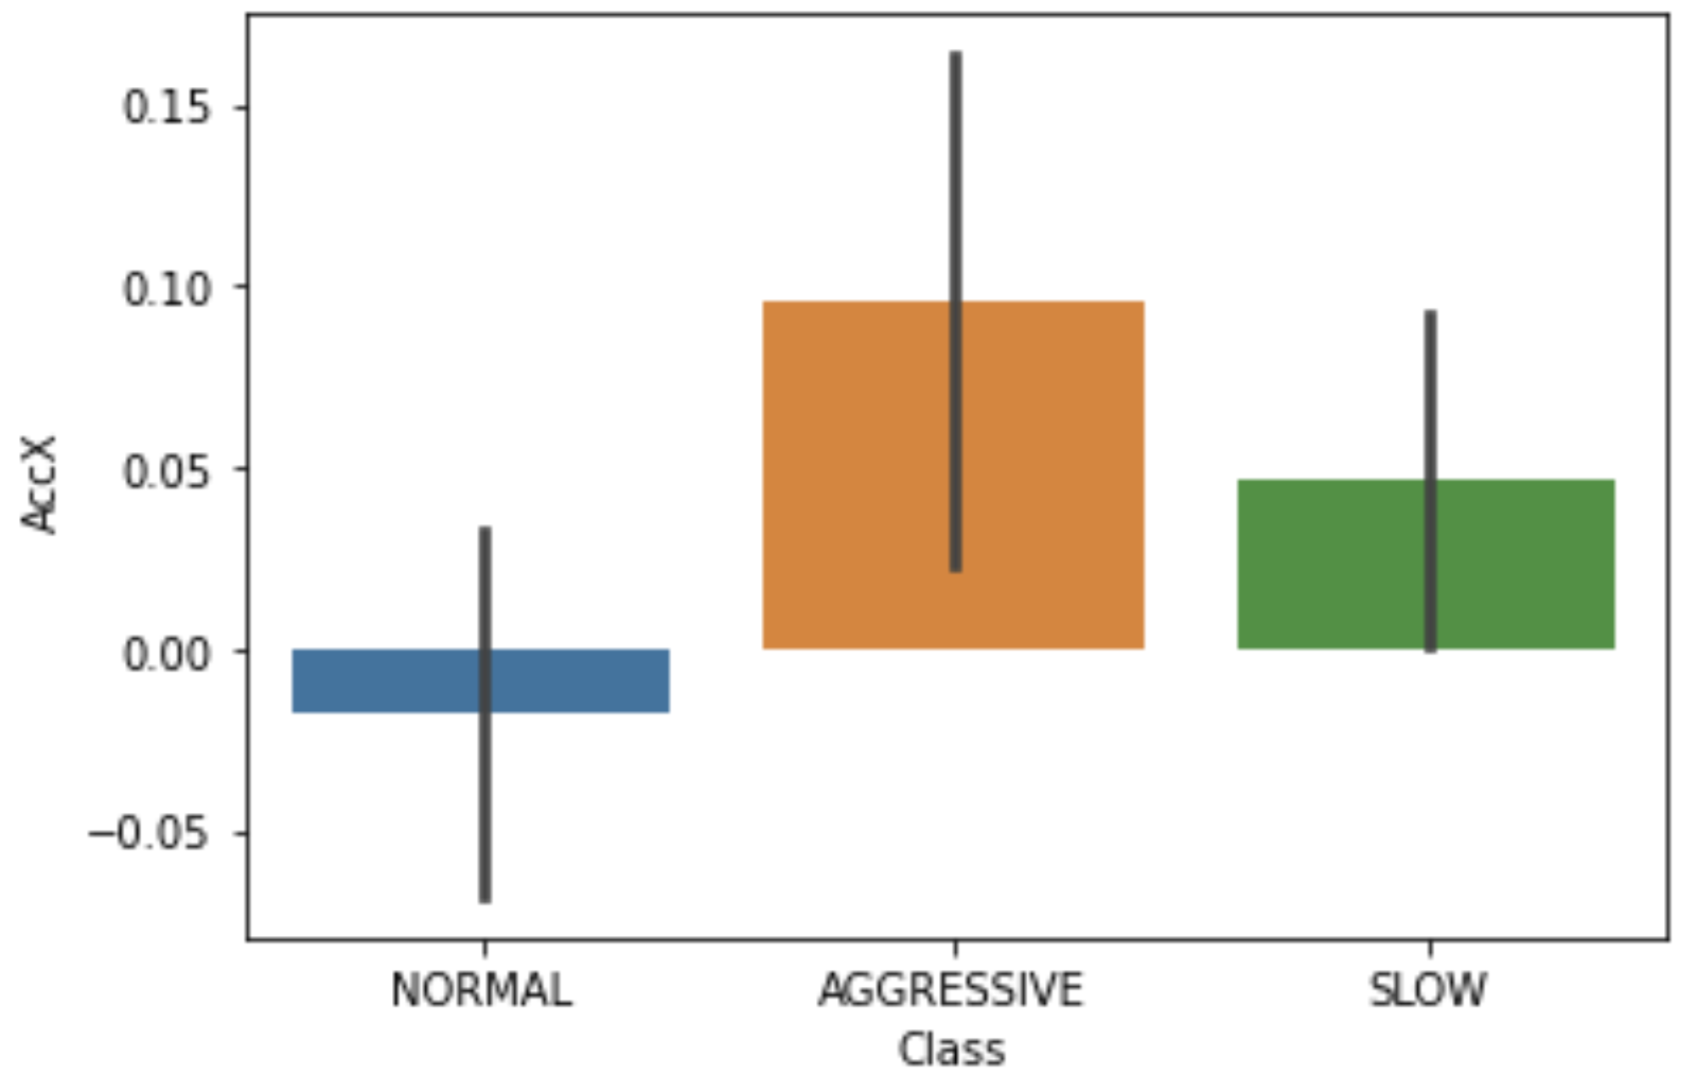
\includegraphics[width=1\columnwidth]{AccX.png}
        \caption{Gráfico comparativo de aceleración en X para las tres clases de comportamiento.}
        \label{fig:comand}%puede ir el nombre que quiera, es solo referencia
    \end{figure}

    \begin{figure}[H]
        \centering
        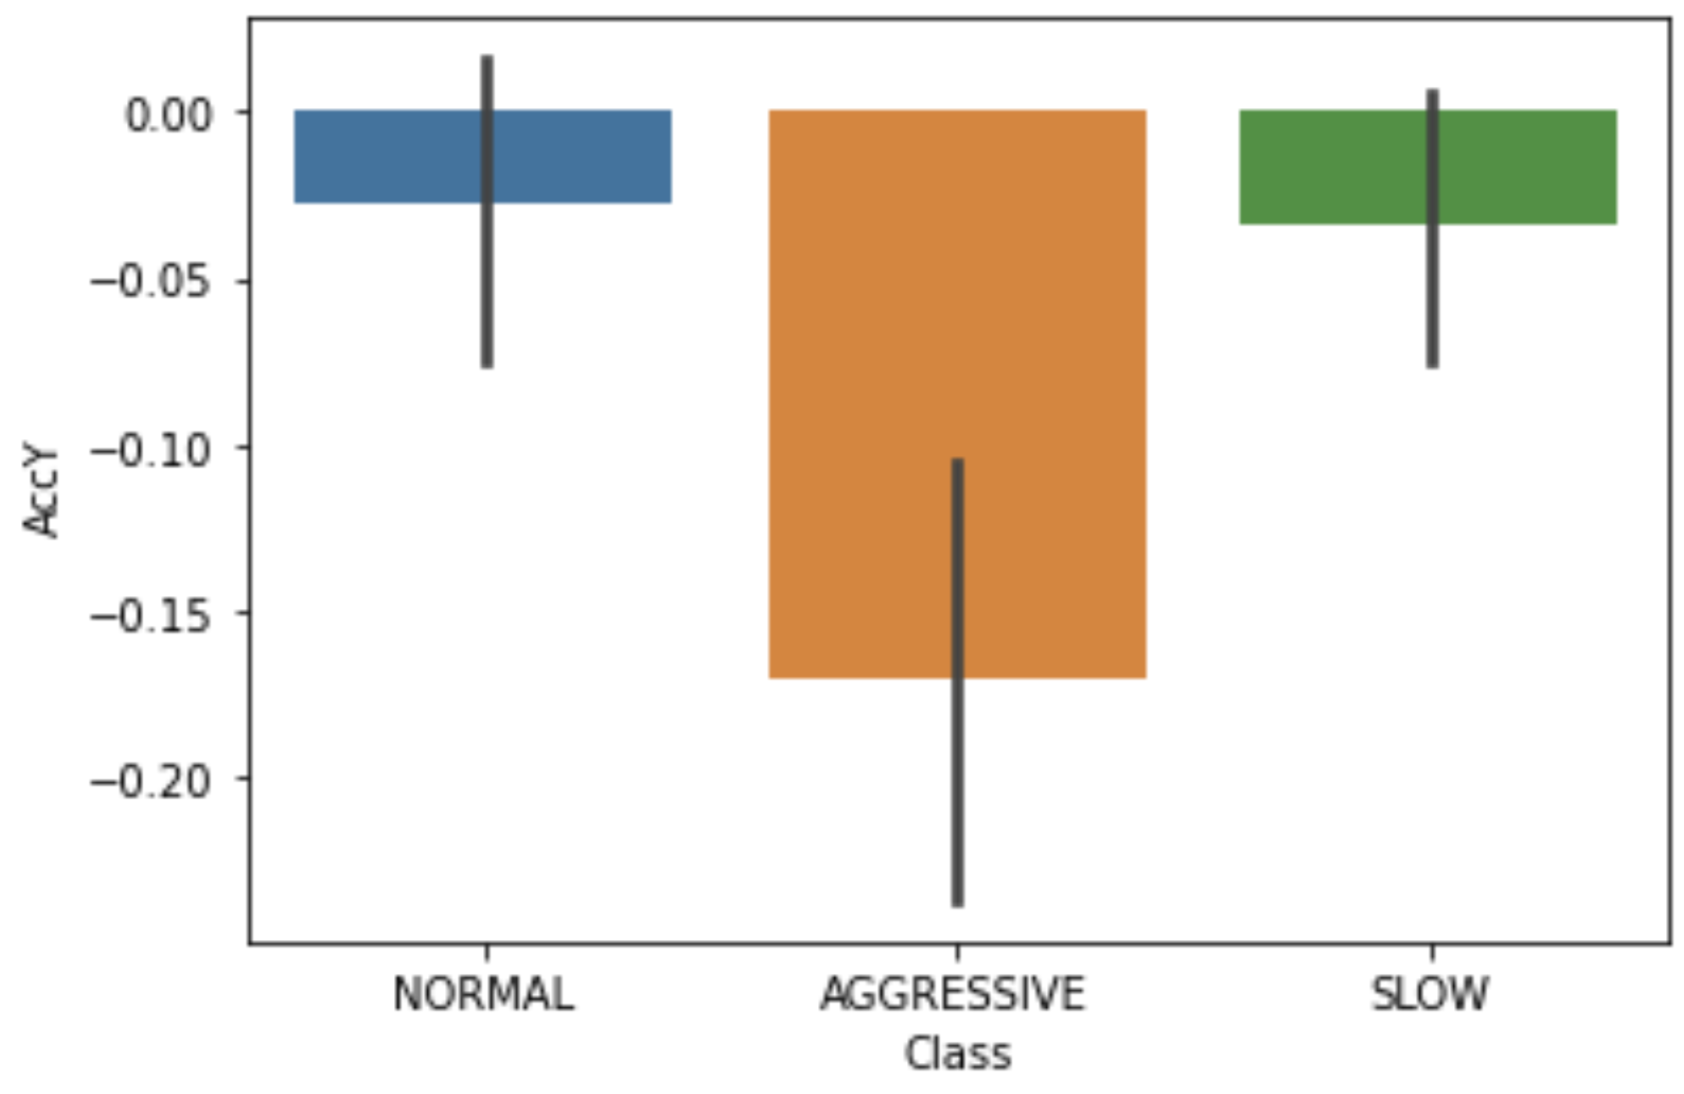
\includegraphics[width=1\columnwidth]{AccY.png}
        \caption{Gráfico comparativo de aceleración en Y para las tres clases de comportamiento.}
        \label{fig:comand}%puede ir el nombre que quiera, es solo referencia
    \end{figure}

    \begin{figure}[H]
        \centering
        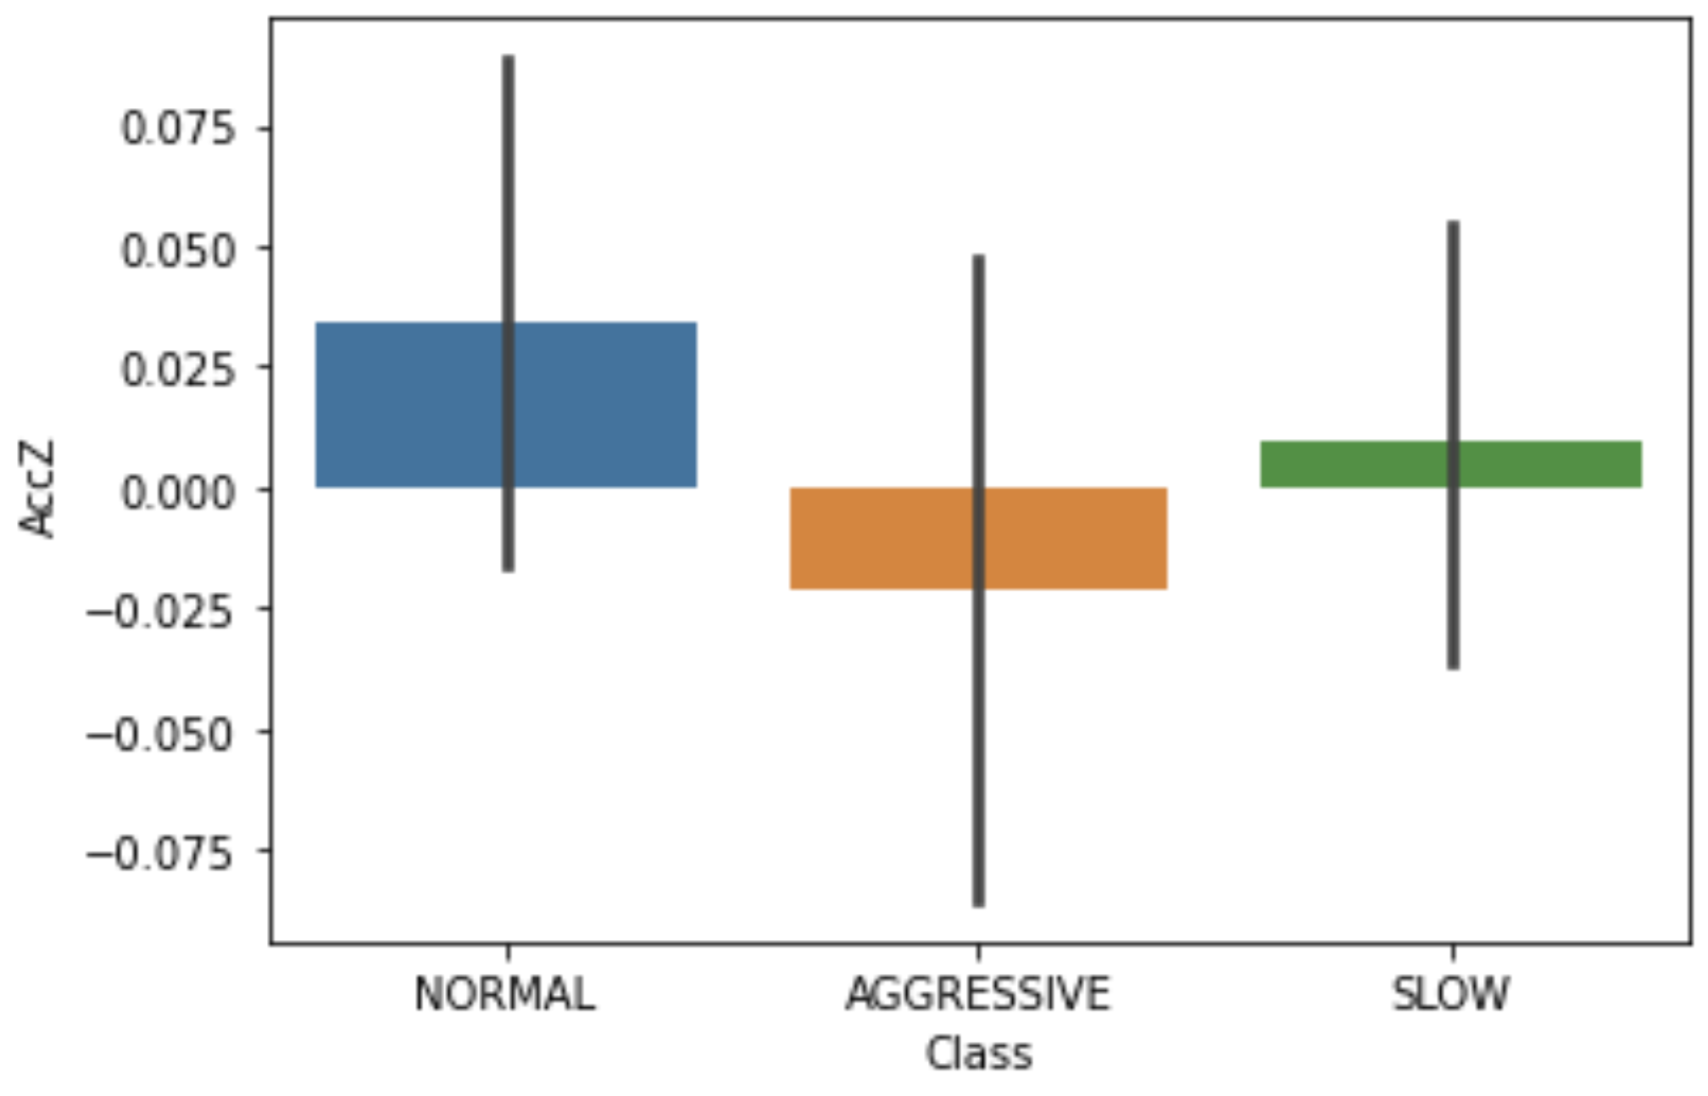
\includegraphics[width=1\columnwidth]{AccZ.png}
        \caption{Gráfico comparativo de aceleración en Z para las tres clases de comportamiento.}
        \label{fig:comand}%puede ir el nombre que quiera, es solo referencia
    \end{figure}

    \begin{figure}[H]
        \centering
        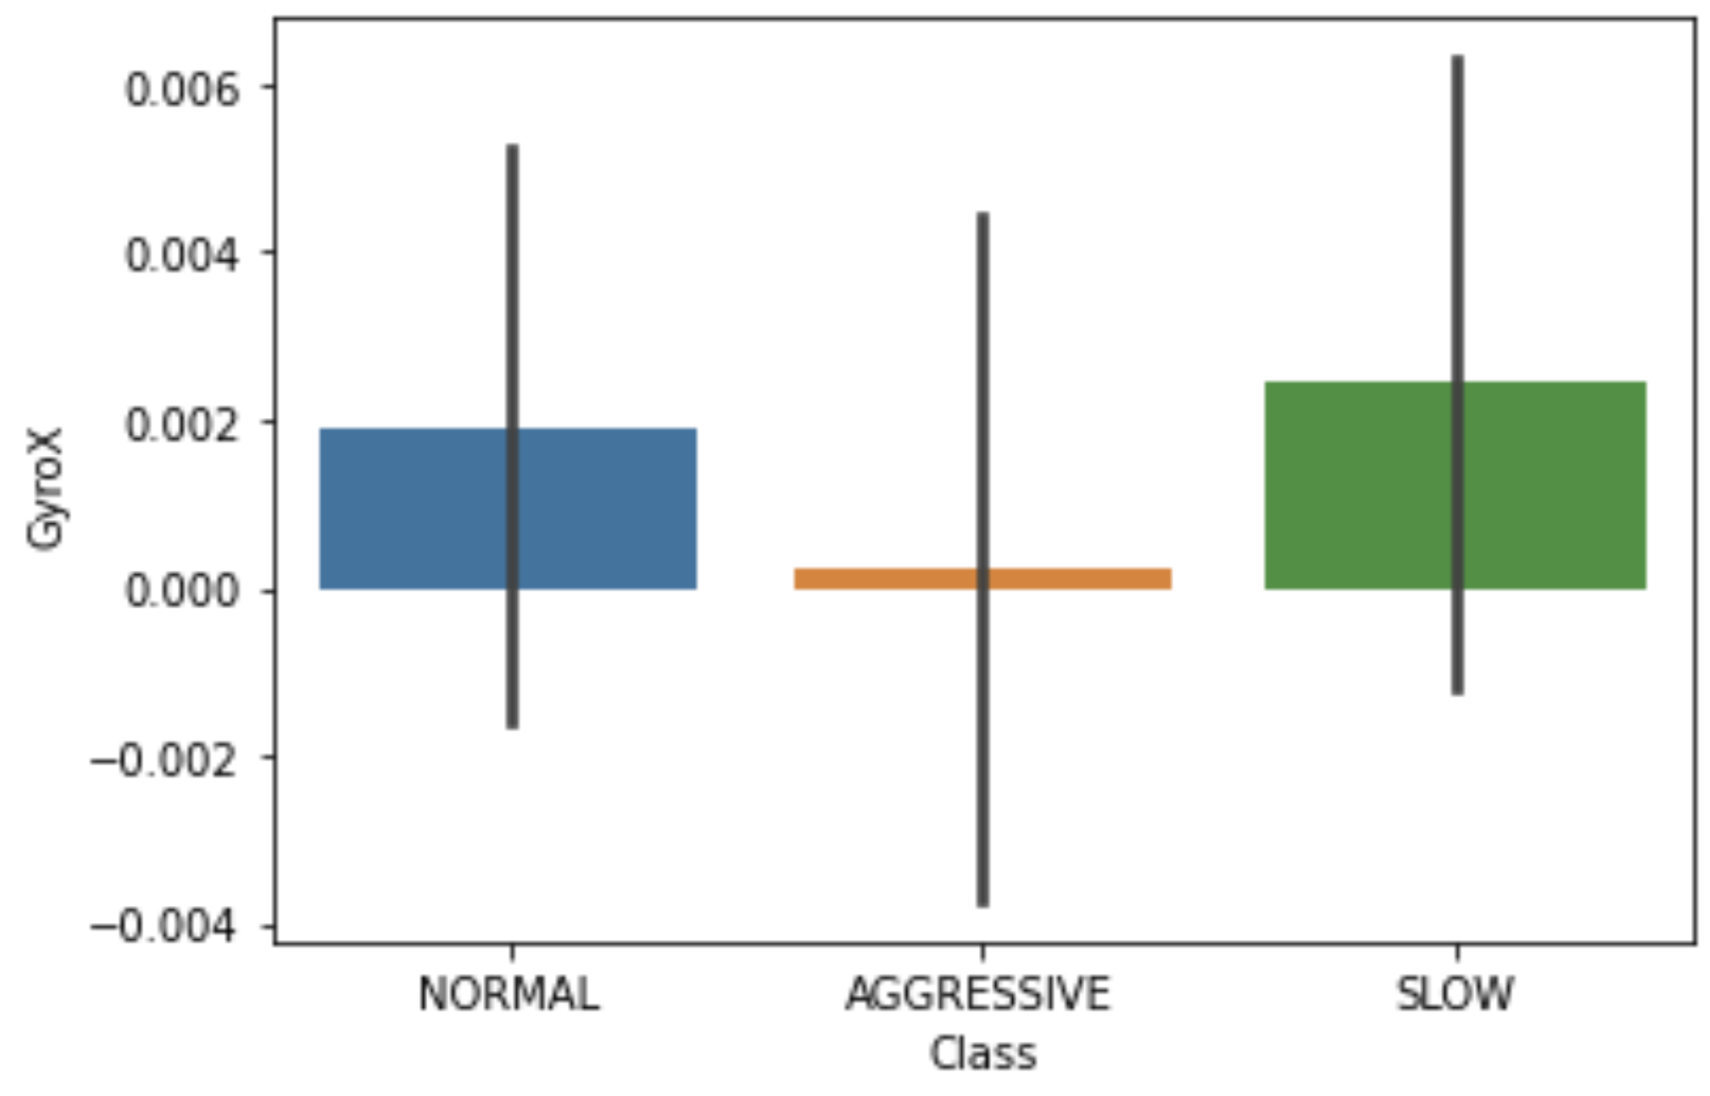
\includegraphics[width=1\columnwidth]{GyroX.png}
        \caption{Gráfico comparativo de giro en X para las tres clases de comportamiento.}
        \label{fig:comand}%puede ir el nombre que quiera, es solo referencia
    \end{figure}

    \begin{figure}[H]
        \centering
        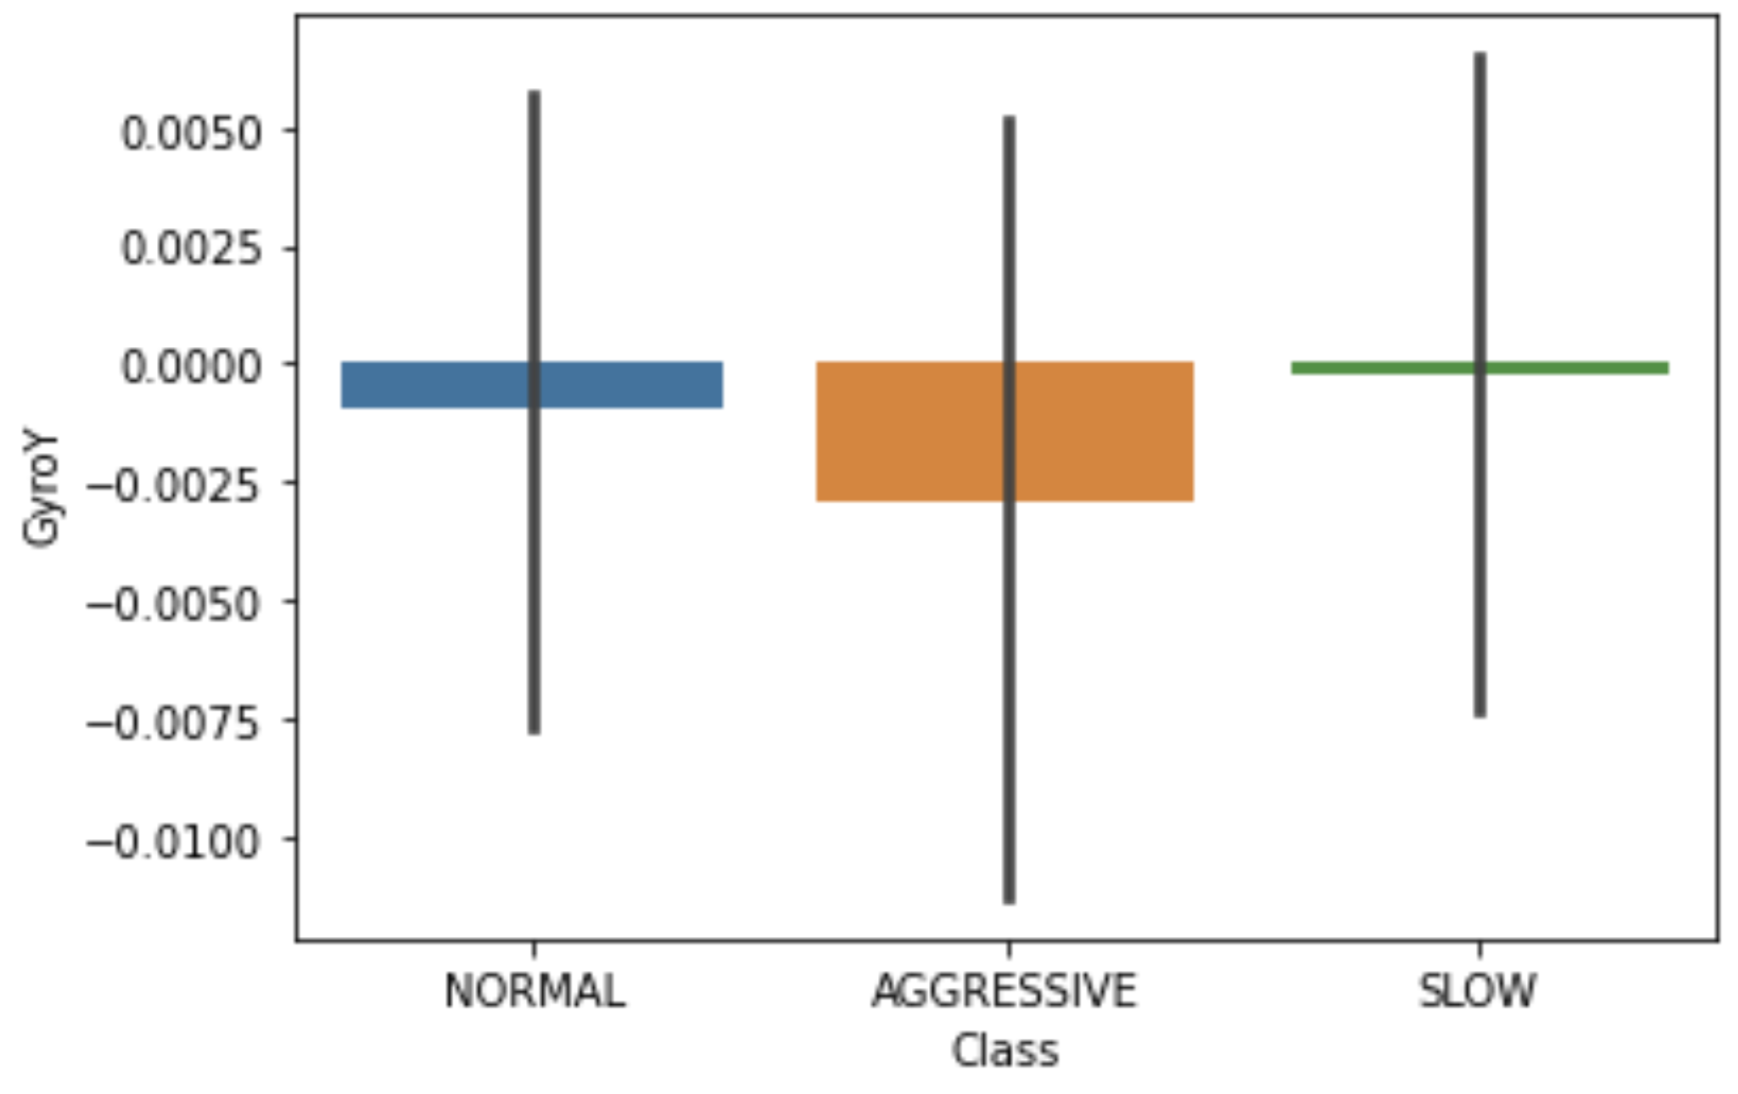
\includegraphics[width=1\columnwidth]{GyroY.png}
        \caption{Gráfico comparativo de giro en Y para las tres clases de comportamiento.}
        \label{fig:comand}%puede ir el nombre que quiera, es solo referencia
    \end{figure}

    \begin{figure}[H]
        \centering
        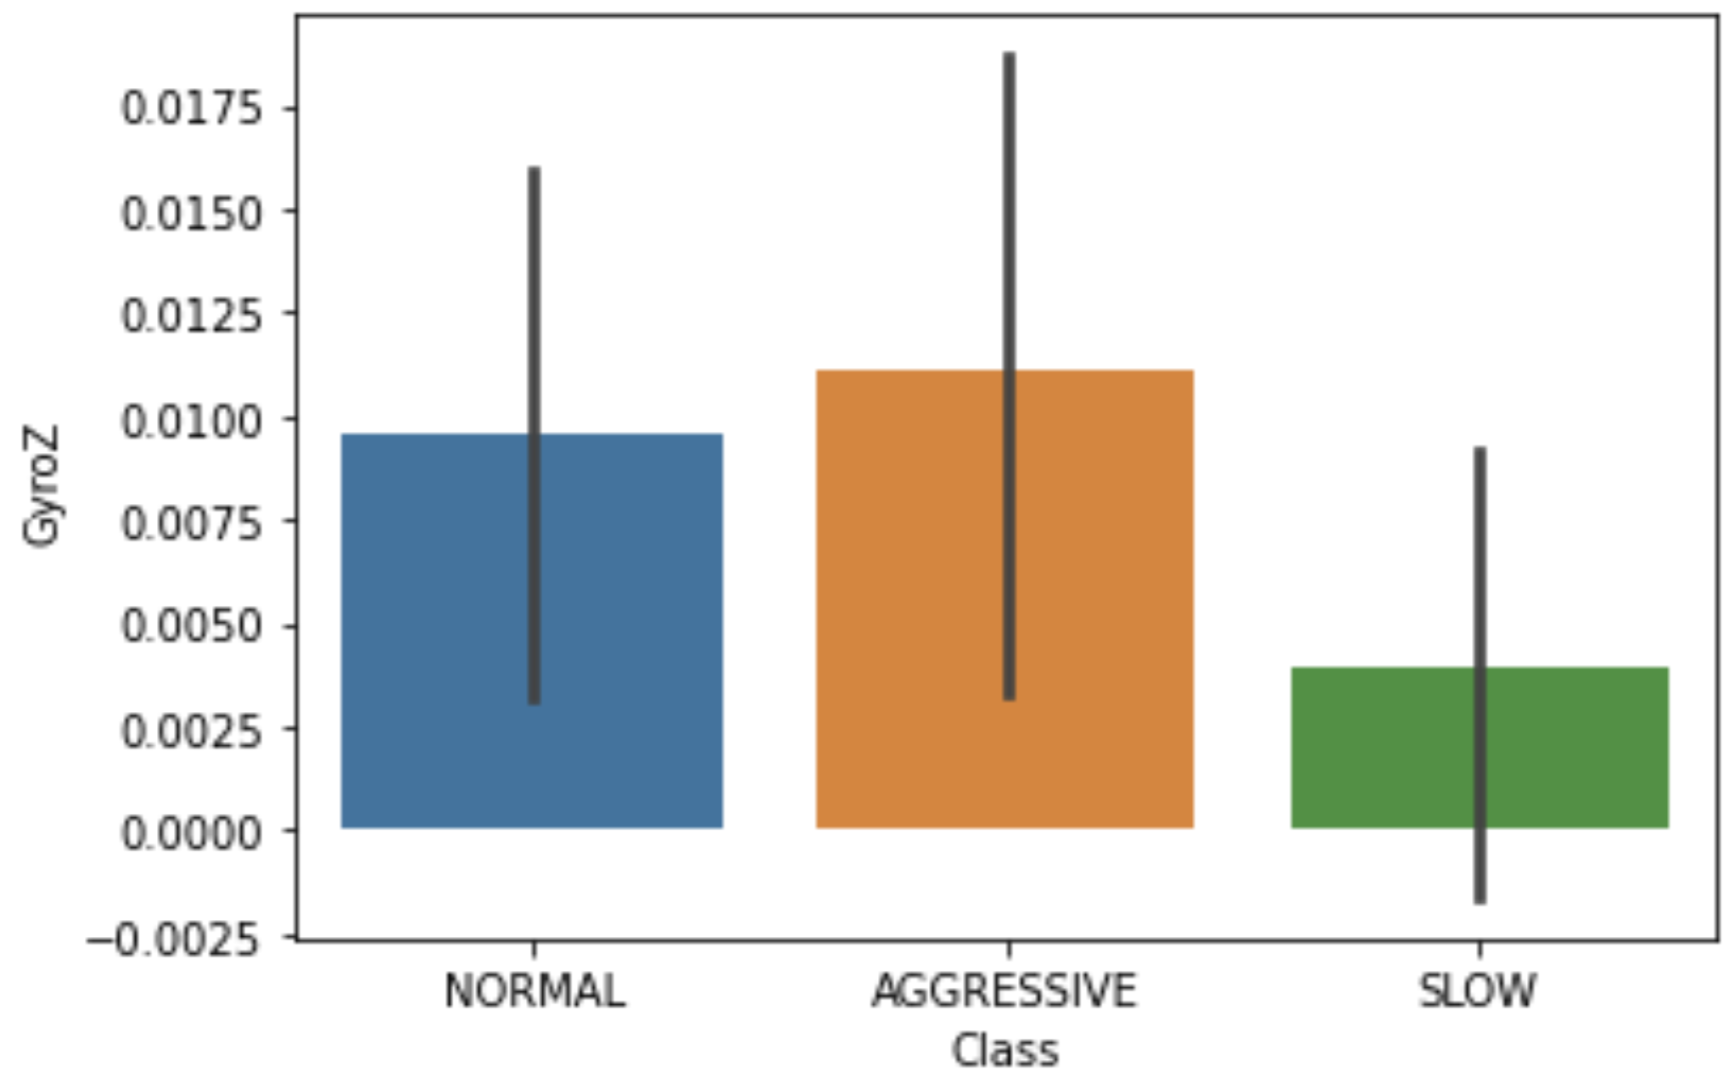
\includegraphics[width=1\columnwidth]{GyroZ.png}
        \caption{Gráfico comparativo de giro en Z para las tres clases de comportamiento.}
        \label{fig:comand}%puede ir el nombre que quiera, es solo referencia
    \end{figure}

\textsc Al observar las gráficas anteriores, podemos darnos cuenta de que realmente podría ser una buena aproximación el hecho de unir las conductas de manejo lentas y normales en una sola categoría, ya que parece que los valores sí hacen una distinción interesante cuando se trata de conductas agresivas. \\

\textsc Una vez realizados estos análisis, se optó por realizar una normalización de los datos para optimizar su manejo en los distintos modelos a implementar y se eliminaron los registros atípicos de las variables independientes, en aras de obtener una mejor precisión en la predicción del comportamiento mediante un modelo óptimo.

\section{Métodos de implementación}
\begin{itemize}
    \item K-Nearest Neighbors
    El algoritmo de K-vecinos más cercanos, por su traducción al español, es uno de los algoritmos más comúnmente usados dentro del aprendizaje de máquina, o \textit{machine learning}, debido a que el modelo es muy simple de implementar y rápido en cuestión de cómputo, resolviendo problemas de clasificación. Este modelo es un método de clasificación supervisada no paramétrico, sirviendo para estimar la función de densidad $F(x/C_j)$ de las predictoras $x$ por cada clase $C_j$, otorgando la probabilidad de que un elemento $x$ pertenezca a a la clase $C_j$ en un rango de $k$ número de vecinos alrededor del elemento a evaluar, contando qué vecino es el que se repite más en el rango especificado por el usuario que realiza el modelo.
    \begin{figure}[H]
        \centering
        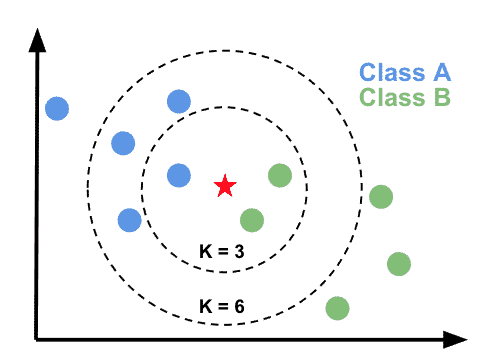
\includegraphics[width=1\columnwidth]{kNN_Neighbors.png}
        \caption{Ejemplo de funcionamiento de K-Nearest Neighbors.}
        \label{fig:comand}%puede ir el nombre que quiera, es solo referencia
    \end{figure}
    
    \item Logistic Regression Algorithm
    El algoritmo de regresión logística, por su traducción al español, es un algoritmo que está relacionado con el área de estadística, usándose en problemas de clasificación binaria |con dos clases posibles|. Este algoritmo parte del uso de la función logística, |conocida también como función sigmoidal|, que se representa con una curva con forma de S que puede tomar cualquier número o valor real y mapearlo o convertirlo en un valor de rango entre 0 y 1 sin incluir dichos limites, siendo su función: $1 / (1 + e^-value)$, donde $e$ es la base de los logaritmos naturales y $value$ es el valor numérico que se busca transformar.
    La regresión logística es representada por una ecuación similar a la regresión linear, donde los valores de entrada $(x)$ se combinan linealmente usando pesos o valores de coeficiente |representados como betas con subíndice n| para predecir un valor de salida $(y)$, que está entre los rangos de 0 y 1. Un ejemplo de una ecuación de regresión logística es: $y = e^(b_0 + b_1*x) / (1 + e^(b_0 + b_1*x))$, donde $b0$ es el intercepto y $b_1$ o $b_n$ es el coeficiente de la variable $x_n$. Gracias a este modelo se puede conocer la probabilidad de pertenencia a una clase en específico, representado como $P(X) = P(Y=1|X)$, donde obtenemos dicha probabilidad con base en un valor de entrada $x$, y se es capaz de predecir, por ende, los valores de salida $y$.
    \begin{figure}[H]
        \centering
        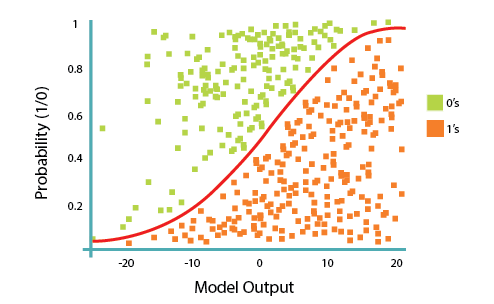
\includegraphics[width=1\columnwidth]{Regresion_Logistica.png}
        \caption{Ejemplo de gráfica de regresión logística.}
        \label{fig:comand}%puede ir el nombre que quiera, es solo referencia
    \end{figure}
    
    \item Random Forest Algorithm:\\
    El algoritmo de árboles aleatorios, por su traducción al español, es uno de los algoritmos más comúnmente usados, debido a que es muy versátil: puede usarse para resolver problemas tanto de regresión como de clasificación. Para explicar su funcionamiento, de manera breve, podemos remitirnos a su nombre: en efecto, el algoritmo construye varios árboles en su interior. Cada árbol tendrá el mismo objetivo: tomar una decisión respecto al problema planteado, ya sea elegir una clase o predecir un valor. Los árboles de decisión son estructuras simples, pero poderosas, que son capaces de elegir una salida tomando en cuenta todas las ramificaciones que las características de cada conjunto de datos otorga. Para ejemplificarlo mejor, tomemos como referencia un conjunto de datos que contiene tres variables independientes: \textit{workToDo, outlook} y \textit{friendsBusy}, con una variable de salida: \textit{whatToDo}. Para determinar la salida de dicha variable, hemos de construir un árbol que incluya todas las posibles combinaciones de decisión de las tres variables independientes. Un ejemplo de lo anterior puede observarse en la figura 11:
    \begin{figure}[H]
        \centering
        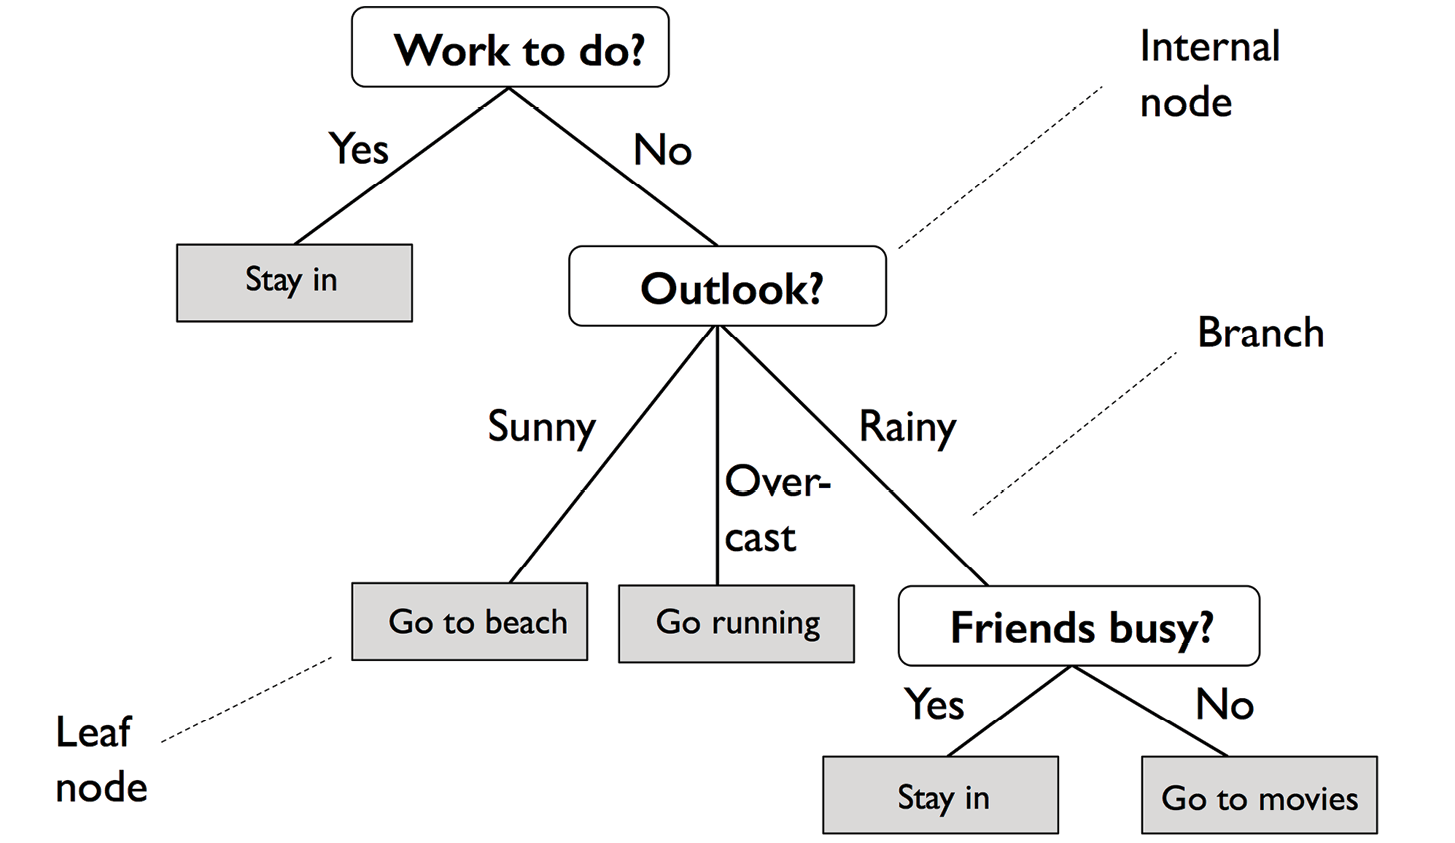
\includegraphics[width=1\columnwidth]{Decision_Tree_Example.jpg}
        \caption{Ejemplo de un árbol de decisión.}
        \label{fig:comand}%puede ir el nombre que quiera, es solo referencia
    \end{figure}
    \\
    En el caso de nuestro conjunto de datos, hemos podido observar en las gráficas comparativas de clases que, en el caso de algunas de ellas, existe una diferencia marcada entre los valores de entrada de ciertas clases: por ejemplo, la aceleración en Z (AccZ), presenta valores negativos al producirse una conducta de manejo agresiva y la aceleración en X (AccX) hace lo mismo con conductas de manejo normales. De esta forma, asumimos, podemos construir un árbol de decisión que nos ayude a determinar la clase de la conducta observada con base en las variables independientes.
    \\
    Adicionalmente, vale la pena destacar que uno de los mayores problemas del uso de árboles de decisión es aquello que conocemos como sobreentrenamiento, un fenómeno en el que el algoritmo aprende demasiado bien lo que sucede con el conjunto de datos de entrenamiento, pero se ajusta tanto que, \textit{a posteriori} le resulta sumamente complejo trabajar con datos fuera de este conjunto de entrenamiento. La aleatoriedad del bosque yace en la elección de variables: se crean conjuntos de variables aleatorias, que, por ende, no se encuentran correlacionadas, lo que contribuye en la significativa disminución del problema tan común que representa el sobreentrenamiento del algoritmo. Es por esto último que hemos decidido usar un bosque aleatorio en lugar de un árbol de decisión unitario, que es más propenso a sufrir de este tipo de problemas.

    \item Multi-Layer Perceptron Classifier
    Un \textit{perceptrón} es una neurona artificial basada en una función matemática de un modelo neuronal biológico $w0(t)$. 
    Es un algoritmo que, a diferencia de otros algoritmos de clasificación, se basa en una red neuronal artificial que puede ser aplicada en problemas no lineales con grandes cantidades de datos y no es necesario tener un gran banco de información para entrenarlo de manera apropiada ya que se puede ajustar y obtener el mismo nivel de precisión que otros algoritmos.\\
    La estructura de este algoritmo consta de:\\
    \begin{itemize}
        \item Datos de entrada
        \item \textit{Hidden layer(s)} |pudiendo ser una o más|.
        \item Datos de salida
    \end{itemize}
    \textit{Funcionamiento:}\\
    El perceptrón, matemáticamente, se describe de la siguiente forma: los datos de entrada se multiplican por los coeficientes de peso, donde el valor puede ser positivo o negativo, de ser positivo |y si el peso previamente calculado supera un umbral establecido|,  la neurona se activa. La predicción se compara con un resultado conocido y de ser erróneo se transmite la información para ajustar los pesos.\\ 
    Esto último no indica que no sea posible sobreentrenar el modelo y que como resultado las predicciones obtenidas con nuevos datos sean erróneas. 
    
    
\end{itemize}

\section{Resultados}
\begin{itemize}
    \item K-Nearest Neighbors:\\
    La implementación del algoritmo K-Nearest Neighbors, con un valor de $k$ = 150, obtuvo una precisión del 74\% y una matriz de confusión de 100\% verdaderos positivos y 99.75\% verdaderos negativos. El reporte de clasificación obtenido se mostrará a continuación en la figura 12. 
    \begin{figure}[H]
        \centering
        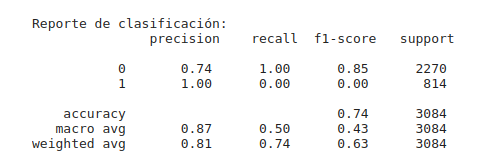
\includegraphics[width=1\columnwidth]{KNN_RC.png}
        \caption{K-Nearest Neighbors - Reporte de clasificación.}
        \label{fig:comand}%puede ir el nombre que quiera, es solo referencia
    \end{figure}
    
    \item Logistic Regression Algorithm:\\
        La implementación del algoritmo de regresión logística obtuvo una precisión del 74\% y una matriz de confusión de 100\% de verdaderos positivos y 100\% de verdaderos negativos. El reporte de clasificación obtenido se mostrará a continuación en la figura 13. 
    \begin{figure}[H]
        \centering
        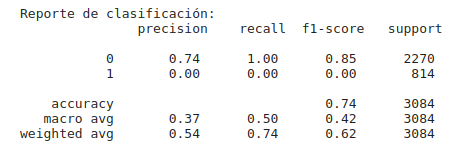
\includegraphics[width=1\columnwidth]{LR_RC.png}
        \caption{Logistic Regression - Reporte de clasificación.}
        \label{fig:comand}%puede ir el nombre que quiera, es solo referencia
    \end{figure}
    
    \item Random Forest Algorithm:\\
    La implementación del bosque aleatorio se dividió en dos fases: aquella en la que se consideraron las tres clases de salida proyectadas en el conjunto de datos original y aquella en la que sólo se consideraron dos clases, uniendo en una sola clase las conductas SLOW y NORMAL de manejo. Para la versión de tres fases, se obtuvo una precisión del 47.21\%, mientras que la segunda tuvo una precisión del 74.35\%. Curiosamente, al observar la matriz de confusión y el reporte de clasificación del algoritmo, en su segunda implementación, que es la que aquí documentaremos, nos percatamos de que el porcentaje de predicción para la clase SLOW-NORMAL es significativamente mayor que la de la clase AGGRESSIVE, por lo que suponemos que el desbalanceo de datos existente en el conjunto, entre ambas clases, podría estar provocando el problema. Al salir de los alcances del bloque TC3006C.101, no realizamos el balanceo de datos con el conjunto computado de prueba, pero, \textit{a posteriori}, podría implementarse esta mejora, en aras de observar si contribuye con el mejoramiento de nuestro algoritmo, principalmente al detectar de forma precisa las conductas de conducción agresivas. Esto último es esencial, pues recordemos que es el objetivo primario de nuestro análisis y, si observamos la matriz de confusión con detenimiento y un poco de sentido común, podremos deducir que el porcentaje de dicha matriz que debemos enfocarnos en reducir es el de falsos negativos para la clase AGGRESSIVE. Según nuestro reporte, el algoritmo fue capaz de predecir únicamente el 25\% de todos los registros de conductas agresivas, dejando fuera, lógicamente, el 75\% de ellas. Recordemos que obtener un algoritmo que compute y realice predicciones con alta precisión es muy deseable, pero es aún más deseable que dicha precisión se concentre en los resultados más vitales del contexto del problema.
    \\
    \begin{figure}[H]
        \centering
        \includegraphics[width=1\columnwidth]{Reporte_de_clasificación_Random_Forest.png}
        \caption{Random Forest - Reporte de clasificación y precisión.}
        \label{fig:comand}%puede ir el nombre que quiera, es solo referencia
    \end{figure}
    \\
    \begin{figure}[H]
        \centering
        \includegraphics[width=1\columnwidth]{Matriz_de_confusión_Random_Forest.png}
        \caption{Random Forest - Matriz de confusión.}
        \label{fig:comand}%puede ir el nombre que quiera, es solo referencia
    \end{figure}

    \item Multi-Layer Perceptron Classifier:\\
    Cuando implementamos el modelo de clasificación multi capa primero establecemos las 4 entradas (AccX, AccY, GyroX, GyroY), 256 hidden layers y 3 resultados (SLOW, NORMAL, AGGRESSIVE). Los resultados de precisión oscilan entre 0.36\% y 0.42\%    
    
\end{itemize}

\section{Discusión}
    Al visualizar los resultados obtenidos por medio de los algoritmos implementados para predecir el tipo de comportamiento de manejo, podemos observar que todos ellos tienen medidas de precisión general similares. Elegiremos el algoritmo de Random Forest, debido a que tuvo una precisión total de 74\% al momento de predecir los valores de salida con base en los datos de entrada. Adicionalmente, el modelo ha sido capaz de predecir correctamente el 25\% de todos los registros del conjunto de datos de prueba que tienen una salida real AGGRESSIVE, por lo que cuenta con el mayor índice de precisión para esta clase, que es la más relevante del problema, por las razones anteriormente descritas.

\section{Conclusión}
Una de las características del reto planteado que vale la pena mencionar en este apartado, es el hecho de que la recolección de los datos podría no ser del todo objetiva. A reservas de indagar aún más en el experimento en el que se recolectaron los datos, todo parece indicar que las conductas de manejo fueron simuladas, por lo que es probable que no reflejen tan fielmente las métricas de conducción correspondientes y se encuentren un poco sesgadas. No obstante, creemos que los resultados obtenidos sí podrían resultar relevantes en el desarrollo de la aplicación que se plantea, aunque, de forma deseable, sería un buen ejercicio futuro el de recolectar datos de conducción en escenarios reales, que colaboren con la investigación.
Por otro lado, el desbalanceo de los datos antes mencionado y su repercusión en el modelo también es un factor importante en el análisis de nuestros resultados, pues ya se ha podido observar que el hecho de que se compute una precisión general del modelo aceptable, podría no significar necesariamente obtener tanta precisión para predecir ciertos aspectos que son, cabe decirlo, aún más relevantes que otros, en vista de que es esencial predecir la mayor cantidad de registros de conductas agresivas que sean posibles.
Finalmente, podemos mencionar la increíble cantidad de cosas aprendidas durante estas cinco semanas, durante las cuales hemos ido descubriendo la importancia de la Ciencia de Datos y sus aplicaciones de una forma interesante y de valor. Este reto nos ha brindado la oportunidad de poner a prueba nuestros conocimientos y nuestra capacidad de inferencia, algo esencial en el quehacer ingenieril.
\end{document}